\documentclass[11pt]{article}

%\usepackage[nosol]{optional}
\usepackage[sol]{optional}

\usepackage {tikz}
    \usetikzlibrary{calc,shapes,arrows,automata,positioning,cd}
    \tikzset{
     dot node/.style={font=\sffamily\small},
      cfgedge/.style   = {black, ->, >=stealth},
      forward/.style = { blue, ->, >=angle 45},
      backward/.style = { red, densely dashed, ->, >=latex' },
      backwardleft/.style = { red, densely dashed, <-, >=latex' },
      position/.style args={#1:#2 from #3}{
        at=(#3.#1), anchor=#1+180, shift=(#1:#2)
    },
    }
    \usepackage{xcolor}

\usepackage{listings, ../listings-rust/listings-rust}
\usepackage{listings}
\usepackage{xcolor}
\definecolor{codegreen}{rgb}{0,0.6,0}
\definecolor{codegray}{rgb}{0.5,0.5,0.5}
\definecolor{codepurple}{rgb}{0.58,0,0.82}
\definecolor{backcolour}{rgb}{0.95,0.95,0.92}
\lstset{
    language=Python,
    keepspaces=true,
    numbers=left,
    backgroundcolor=\color{backcolour},
    commentstyle=\color{codegreen},
    basicstyle=\ttfamily,
    otherkeywords={self,True,False,yield},
    keywordstyle=\ttfamily\color{blue!90!black},
    %basicstyle=\footnotesize,
    keywords=[3]{ttk},
    keywordstyle={[2]\ttfamily\color{orange!80!orange}},
    keywordstyle={[3]\ttfamily\color{red!80!orange}},
    emph={MyClass,__init__},
    emphstyle=\ttfamily\color{red!80!black},
    stringstyle=\color{green!80!black},
    showstringspaces=false
}

\newcommand{\N}{\mathbb{N}}
\newcommand{\Z}{\mathbb{Z}}

% For proof.
\usepackage{amsmath,amsthm,amssymb}

\usepackage{enumerate}
\usepackage{graphicx}
\usepackage{float}
\usepackage{subcaption}
\usepackage{comment}

\renewcommand{\topfraction}{.9}
\renewcommand{\textfraction}{.1}

\usepackage{fullpage,amsmath,amssymb}
\usepackage[colorlinks=true,citecolor=blue,linkcolor=blue]{hyperref} % for href links, and also makes \ref and \eqref clickable in the PDF

% parenthetical comment to state verbally but not write on the board
\newcommand{\com}[1]{\footnote{#1}}

\newcommand{\deltahat}{\widehat{\delta}}

\newcommand{\QuasiP}{\mathsf{QuasiP}}

\newcommand{\TIME}{\mathsf{TIME}}

\usepackage{fancyhdr}
\fancypagestyle{firststyle}
{
    \fancyhf{}
    \fancyhead[C]{Copyright \copyright\ \today, David Doty}
}


\title{Homework 5 \opt{sol}{Solutions} -- ECS 220, Winter 2020}
\date{}
\begin{document}
\maketitle
\thispagestyle{firststyle}
\vspace{-2.0cm}

\section{Good old-fashioned Geography. (Textbook problem 8.21)}
Now consider really traditional Geography, where the alphabet is limited to, say, 26 symbols.
More formally,
for a directed graph $G=(V,E)$ and alphabet $\Sigma$,
say that $G$ is \emph{$\Sigma$-alphabetic} if there is are functions $f,\ell:V \to \Sigma$
obeying the conditions in the definition of \textsc{Alphabetic-Geography},
and let $\Sigma$\textsc{-Alphabetic-Geography} be the corresponding decision problem asking,
given a $\Sigma$-alphabetic graph $G$ and starting node $v$,
whether Player 1 has a winning strategy starting at $v$.
Show that for each fixed alphabet $\Sigma$,
$\Sigma$\textsc{-Alphabetic-Geography}$\in\mathsf{P}$.

\section{solution} 
Before we start, we recall an intuitive algorithm that can solve the Geography game recursively.\\
Define $check(G,v)$, $G$ is the current-state-graph and $v$ is the next search node: 
\begin{enumerate}[(a)]
    \item If the out-degree of node $v$ = 0, return False.
    \item Remove node $v$, and all the edges that $v$ connected (begin with $\&$ end with), called the current graph $G'$.
    \item For each node $i$ of $v$'s neighbour, $check(G',i)$.
    \item If one of the above $check()$ return False, then return True (meaning that the Player 1 has found a method that Player 2 reaches lose end); else return False.
\end{enumerate}
Then we will show that for each fixed alphabet $\Sigma$,
    $\Sigma$\textsc{-Alphabetic-Geography}$\in\mathsf{P}$.\\
    (There may be some algorithms that run faster, but there we just provide an simple and easy-understandable algorithm that in $\in\mathsf{P}$)\\
    Suppose the finite alphabet $\Sigma$ with $|\Sigma|=k$ and each elements in $\Sigma$ is $\sigma_i, i\in \{1,2,...,k\}$,\\
    We mark each node $v$ with its $(f(v),l(v))$, $f(v),l(v)\in \Sigma$.\\
    So there are total $|V|=n$ nodes with at most $k^2$ kinds, that is, for all the nodes that marked as $(\sigma_i,\sigma_j)$, they share all the same edges in and out with other nodes. For instance, since it is a strictly Alphabetic-Geography graph, all the node marked as $(\sigma_i,\sigma_j)$ will have out-coming edges with nodes that $f(v)=\sigma_j$ and in-coming edges with nodes that $l(v)=\sigma_i$.\\
    So, we can build the recursive function tree, see below:\\
    Since for each node, before we do the recursion we will remove itself and all the edges that it connected (begin with $\&$ end with). And we know that for the combination $k^2=|f(v)|*|l(v)|$ there are at most $k^2$ depths of the recursive tree. And for each layer there are at most $N$ nodes, so the final time complexity of this recursive algorithm is $O(n^{k^2})$, which is polynomial time complexity.
    \begin{figure}[h]
    \centering
    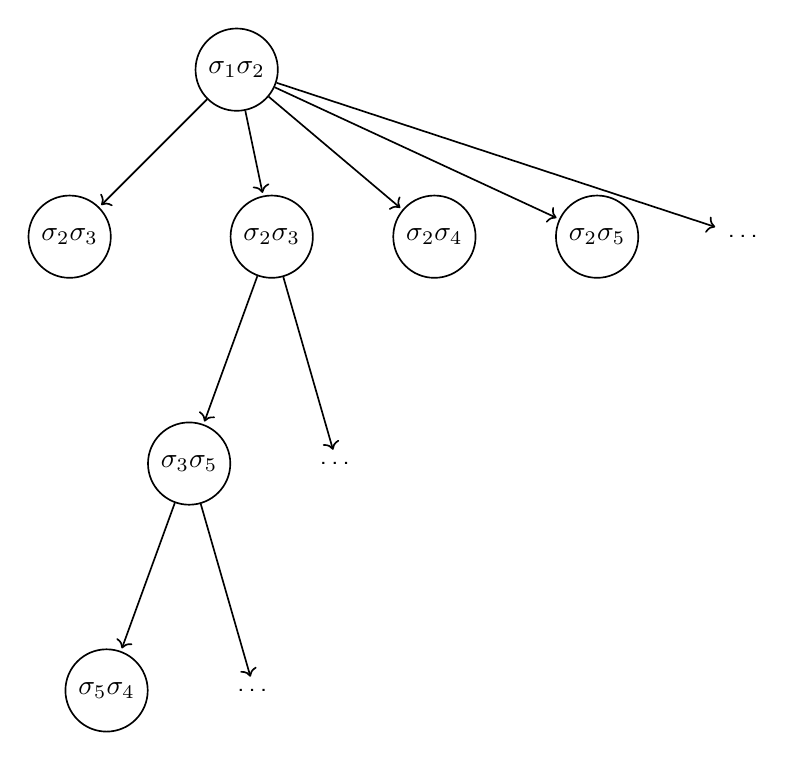
\begin{tikzpicture}[shorten >=1pt,node distance=3cm,on grid,auto, semithick]
        \node [state] (a)   {$\sigma_1\sigma_2$};
        \node [state] (b) [below left of=a]  {$\sigma_2\sigma_3$};
        \node [state] (c) [position=0: 1.5cm from b]  {$\sigma_2\sigma_3$};
        \node [state] (d) [position=0: 1cm from c]  {$\sigma_2\sigma_4$};
        \node [state] (e) [position=0: 1cm from d]  {$\sigma_2\sigma_5$};
        \node [dot node] (f) [position=0: 1cm from e]  {\ldots};
        \node [state] (g) [position=250: 2cm from c]  {$\sigma_3\sigma_5$};
        \node [dot node] (h) [position=0: 1cm from g]  {\ldots};
        \node [state] (i) [position=250: 2cm from g]  {$\sigma_5\sigma_4$};
        \node [dot node] (j) [position=0: 1cm from i]  {\ldots};
        \path[->]
        (a) edge (b)
        (a) edge (c)
        (a) edge (d)
        (a) edge (e)
        (a) edge (f)
        (c) edge (g)
        (c) edge (h)
        (g) edge (i)
        (g) edge (j);
    \end{tikzpicture}
    \caption{The recursive tree}
\end{figure}

\end{document}
